\documentclass[10pt]{article}
\usepackage[fontsize=10pt]{fontsize}

\usepackage[margin=0.5in]{geometry} 
\usepackage{amsmath,amsthm,amssymb, graphicx, multicol, array, txfonts}
\usepackage{bbm}
\usepackage{hyperref}
\hypersetup{
    colorlinks=true,
    linkcolor=blue,
    filecolor=magenta,      
    urlcolor=cyan,
    pdftitle={Overleaf Example},
    pdfpagemode=FullScreen,
    }

\urlstyle{same}


\newcommand{\N}{\mathbb{N}}
\newcommand{\Z}{\mathbb{Z}}
\setcounter{secnumdepth}{0}
\setlength\parindent{0pt}

 
\newenvironment{problem}[2][Problem]{\begin{trivlist}
\item[\hskip \labelsep {\bfseries #1}\hskip \labelsep {\bfseries #2.}]}{\end{trivlist}}

\newenvironment{prelim}[2][Preliminaries]{\begin{trivlist}
\item[\hskip \labelsep {\bfseries #1}\hskip \labelsep {\bfseries #2}]}{\end{trivlist}}
    
\begin{document}
 
\title{6.S091: Problem Set 3}
\author{Suyeol Yun\\
syyun@mit.edu}
\maketitle
 
\section{Problem 1: Constructing Minimal I-MAPs [5 points]}
* Code is available at \url{https://github.com/syyunn/6.S091/blob/main/pset3/pb1.py}

\subsection{(a)} 
1. Draw $\mathcal{G}_{\pi_a}$\\

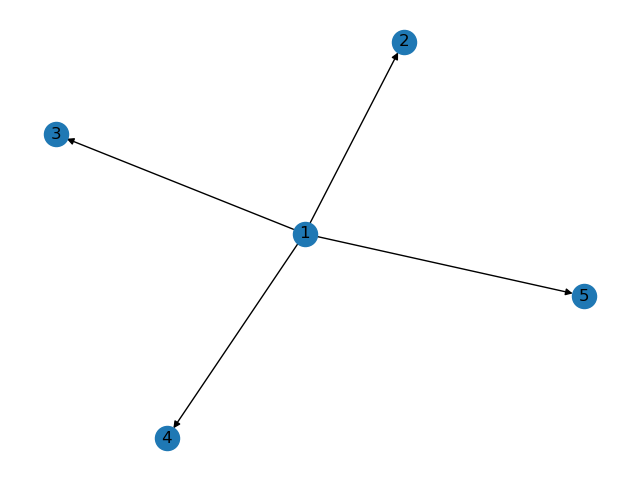
\includegraphics{images/pb1a.png}

2. Draw $\mathcal{G}_{\pi_b}$\\

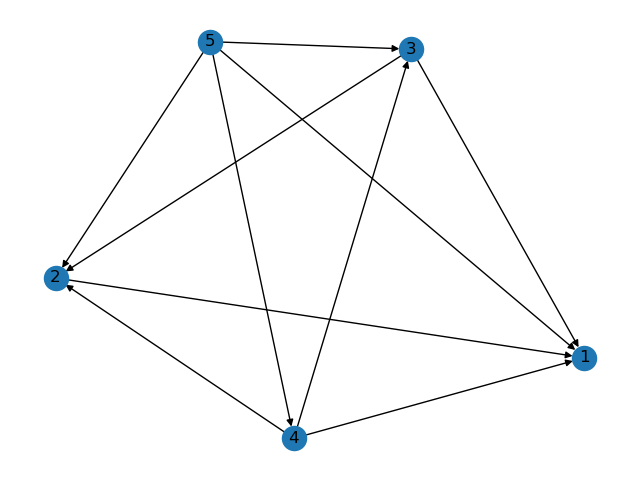
\includegraphics{images/pb1b.png}

3. Draw $\mathcal{G}_{\pi_c}$\\

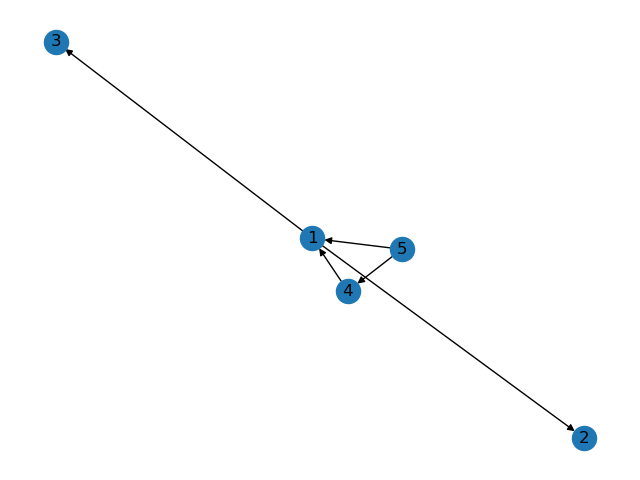
\includegraphics{images/pb1c.png}

\subsection{(b)}
We can transform  $\mathcal{G}_{\pi_a}$ into $\mathcal{G}_{\pi_c}$ by the Chickering sequence (Add $5 \rightarrow 4$, Reverse $1\rightarrow 5$, then Reverse $1\rightarrow 4$).

\section{Problem 2}
\subsection{(a)}
Let $\gamma_m$ be an arbitrary node of the d-connecting path $\gamma$. Since $\gamma$ is d-connected, $\gamma_m$ is unblocked over the path from $A \in \mathbf{A}$ to $B \in \mathbf{B_1}$ given $\mathbf{S} \cup \mathbf{B_2}$. Since $\gamma_m$ is unblocked, $\gamma_m$ is either a non-collider or a collider. 
First, if $\gamma_m$ is a non-collider, $\gamma_m \notin \mathbf{S} \cup \mathbf{B_2}$ and it implies $\gamma_m \notin \mathbf{S}$, which implies that $\gamma_m$ is unblocked over the path from $A \in \mathbf{A}$ to $B \in \mathbf{B}$ given $\mathbf{S}$ because $B \in \mathbf{B_1} \subset \mathbf{B}$.
Second, if $\gamma_m$ is a collider, 
then $\overline{\text{de}}_\mathcal{G}(\gamma_m) \cap \left(\mathbf{S} \cup \mathbf{B_2}\right)\neq\emptyset$. 
Let $\zeta_m \in \overline{\text{de}}_\mathcal{G}(\gamma_m)$ be the closest node to $\gamma_m$ among the nodes in $\overline{\text{de}}_\mathcal{G}(\gamma_m) \cap \left(\mathbf{S} \cup \mathbf{B_2}\right)$. 
Then $\zeta_m$ is either in $\mathbf{S}$ or in $\mathbf{B_2}\setminus \mathbf{S}$.
If $\zeta_m \in \mathbf{S}$, $\gamma_m$ is unblocked over the path from $A \in \mathbf{A}$ to $B \in \mathbf{B}$ given $\mathbf{S}$ because $\overline{\text{de}}_\mathcal{G}(\gamma_m) \cap \mathbf{S}\neq\emptyset$.
If $\zeta_m \in \mathbf{B_2\setminus S}$, any nodes over the decendent path between $\gamma_m$ to $\zeta_m$ are not in $\mathbf{S}$ thus they are unblocked over the path from $A \in \mathbf{A}$ to $\zeta_m \in \mathbf{B_2} \subset \mathbf{B}$ given $\mathbf{S}$ because they are non-colliders and they are not in $\mathbf{S}$.
Therefore, we can always find a d-connecting path $\gamma'$ between $A \in \mathbf{A}$ and $B' \in \mathbf{B}$ given $\mathbf{S}$.

\subsection{(b)}
$B$ can be either in $\mathbf{B_1}$ or $\mathbf{B_2}$. If $B \in \mathbf{B_2}$, then the path $\gamma$ can be a d-connecting path $\gamma'$ from $A \in \mathbf{A}$ to $B' \in \mathbf{B_2}$ given $\mathbf{S}$. Otherwise, 
if $B \in \mathbf{B_1}$, let $\gamma_m$ be an arbitrary node of the d-connecting path $\gamma$. 
Then $\gamma_m$ is either non-collider or collider.
If $\gamma_m$ is a collider, 
$\overline{\text{de}}_\mathcal{G}(\gamma_m) \cap \mathbf{S} \neq\emptyset$ which implies 
$\overline{\text{de}}_\mathcal{G}(\gamma_m) \cap \left(\mathbf{S} \cup \mathbf{B_2}\right)\neq\emptyset$ which implies $\gamma_m$ is unblocked over the path from $A \in \mathbf{A}$ to $B \in \mathbf{B_1}$ given $\mathbf{S} \cup \mathbf{B_2}$.
If $\gamma_m$ is non-collider, $\gamma_m \notin \mathbf{S}$. 
If $\gamma_m$ is also not in $\mathbf{B_2}$, then $\gamma_m$ is unblocked over the path from $A \in \mathbf{A}$ to $B \in \mathbf{B_1}$ given $\mathbf{S} \cup \mathbf{B_2}$.
If $\gamma_m$ is not in $\mathbf{S}$ but in $\mathbf{B_2}$, we can shorten the path $\gamma$ by removing the trailing nodes of $\gamma_m$ from $\gamma$. 
This shortened path is d-connecting path $\gamma'$ from $A \in \mathbf{A}$ to $B' \in \mathbf{B_2}$ given $\mathbf{S}$.
Therefore, we can always find a d-connecting path of either one of the given two types.


% Over this shortened node, we can repeat the same argument until we get all nodes to be unblocked
% over the path from $A \in \mathbf{A}$ to $B \in \mathbf{B_1}$ given $\mathbf{S} \cup \mathbf{B_2}$.


\section{Problem 3}
* Code is available at \url{https://github.com/syyunn/6.S091/blob/main/pset3/search_mec.py}

\subsection{(a)}
$\text { starting\_dag2 and 3 }$ both have $4$ neighbors. 
\subsection{(b)}
1. $\text { starting\_dag2}$ has the shortest path of length $1$.\\
2. $\text { starting\_dag3}$ has the shortest path of length $3$.
\end{document}
